\documentclass
[
a4paper,
openright,                    % Kap.beginn immer rechts! (fkt. nur bei report, nicht bei article)
12pt                          % ersatzweise 12pt, wenn mehr Seiten entstehen sollen
]
{report}

%%%%%%%%%%%%%%%%%%%%%%%%%%%%%%%%%%%%%%%%%%%%%%%%%%%%%%%%%%%%%%%%%%%%%%%%%%%%%%%%%%%%%%%%%%%%%%%%%%%%%%%%%%%%
%Dokumenteneigenschaften

\newcommand{\Author}{Mr. Stefan Binna} 
\newcommand{\Title}{Renewal of the IT Infrastructure of the Royal Institute for Tourism \& Hospitality in Thimphu/Bhutan}
\newcommand{\Keywords}{KEYWORD 1, KEYWORD 2, KEYWORD 3, KEYWORD 4, KEYWORD 5}
\newcommand{\Advisor}{DI Norbert Egger}
\newcommand{\Companyadvisor}{Mag. Leonhard W\"orndl}
\newcommand{\Birthdate}{03.12.1993}
\newcommand{\EnrolNum}{1410555001}
\newcommand{\VenueMonthYear}{Thimphu/Bhutan, May 2016}
\newcommand{\VenueDate}{Thimphu, am 01.05.2016}

%%%%%%%%%%%%%%%%%%%%%%%%%%%%%%%%%%%%%%%%%%%%%%%%%%%%%%%%%%%%%%%%%%%%%%%%%%%%%%%%%%%%%%%%%%%%%%%%%%%%%%%%%%%%
% Layout zusammengestellt von Richard Wanger im WS 2015/2016. Verschiedene Vorlagen wurden bei der Erstellung
% kombiniert und nach dem Masterleitfaden (Stand: Oktober 2015) adaptiert. Verwendung ohne Gewähr!

\usepackage{style}		%alle packages und Formatvorlagen befinden sich in dieser Datei


%%%%%%%%%%%%%%%%%%%%%%%%%%%%%%%%%%%%%%%%%%%%%%%%%%%%%%%%%%%%%%%%%%%%%%%%%%%%%%%%%%%%%%%%%%%%%%%%%%%%%%%%%%%%
% ORGANISATORISCHES

\begin{document}
\begin{titlepage}

\hspace{7cm}

\begin{figure}[!ht]
	\centering
	
\includegraphics[width=0.3\textwidth]{fhs_logo_web.png}
\end{figure}

\begin{center}
	\vspace{2cm}
	\Huge Laboratory II
	
	\Large{\bf\large Binna, Reschenhofer, Schörghofer}
	\vspace{1cm}

	\large Course: Internet Infrastructure and Security 
	
	\large Lecturer: FH-Prof. DI Mag. Dr. Dominik Engel 
	
	\large 23.11.2016
\end{center}

%\vfill
\end{titlepage}
%\chapter*{Danksagung}
\thispagestyle{empty}
\pagestyle{empty}

Die Danksagung ist NICHT vorgeschrieben.


\newpage

%%%%%%%%%%%%%%%%%%%%%%%%%%%%%%%%%%%%%%%%%%%%%%%%%%%%%%%%%%%%%%%%%%%%%%%%%%%%%%%%%%%%%%%%%%%%%%%%%%%%%%%%%%%%
%VERZEICHNISSE

\pagenumbering{roman}
\thispagestyle{plain}
\pagestyle{plain}

\tableofcontents
\protect \addcontentsline{toc}{chapter}{Table of Contents}

\renewcommand{\nomname}{List of Abbreviations}
% !TeX root = 00General.tex

\chapter*{List of Abbreviations}
\addcontentsline{toc}{chapter}{List of Abbreviations} 
\pagestyle{plain}

\begin{acronym}[VLAN123]
 \acro{ARP}{Address Resolution Protocol}
 \acro{CD}{Collision Detection}
 \acro{CRC}{Cyclic Redundancy Check}
 \acro{FCS}{Frame Check Sequence}
 \acro{IEEE}{Institute of Electrical and Electronics Engineers}
 \acro{MAC}{Media Access Control}
 \acro{NIC}{Network Interface Card}
 \acro{NTP}{Network Time Protocol}
 \acro{PTP}{Precision Time Protocol}
 \acro{QoS}{Quality of Service}
 \acro{RIP}{Routing Information Protocol}
 \acro{RSTP}{Rapid Spanning Tree Protocol}
 \acro{SAT}{Source Address Table}
 \acro{STP}{Spanning Tree Protocol}
 \acro{USB}{Universal Serial Bus}
 \acro{VLAN}{Virtual Local Area Network}
 \acro{MOTD}{Message of the Day}
 \acro{PVST}{Per-VLAN Spanning Tree}
 \acro{VTP}{VLAN Trunking Protocol}
 \acro{SSH}{Secure Shell}
 \acro{DHCP}{Dynamic Host Configuration Protocol}
 \acro{DCE}{Data Communication Endpoint}
 \acro{OSPF}{Open Shortest Path First}
 \acro{IP}{Internet Protocol}
 \acro{LSR}{Link State Routing}
 \acro{AS}{Autonomous System}
 \acro{TTL}{Time To Live}
 \acro{POP3}{Post Office Protocol Version 3}
 \acro{SMTP}{Simple Mail Transfer Protocol}
 \acro{SSL}{Secure Socket Layer}
 \acro{TLS}{Transport Layer Security}
 \acro{HTTPS}{Hyper Text Transport Protocol Secure}
\end{acronym}


%\listoffigures
%\protect \addcontentsline{toc}{chapter}{List of Figures}

%\listoftables
%\protect \addcontentsline{toc}{chapter}{List of Tables}

%\lstlistoflistings
%\protect \addcontentsline{toc}{chapter}{Listingverzeichnis}

%%%%%%%%%%%%%%%%%%%%%%%%%%%%%%%%%%%%%%%%%%%%%%%%%%%%%%%%%%%%%%%%%%%%%%%%%%%%%%%%%%%%%%%%%%%%%%%%%%%%%%%%%%%%
%INHALT

%\clearpage
%\pagenumbering{arabic}
%\chapter{Beispiele}

\thispagestyle{standard}
\pagestyle{standard}

\section{Text und Zitate}

In Moby-Dick geht es in erster Linie um die Jagd auf einen weißen Pottwal \footnote{nach: https://de.wikipedia.org/wiki/Moby-Dick}. Kurze Zitate (unter drei Zeilen) müssen mit Anführungszeichen gekennzeichnet werden. Außerdem müssen die Quelle sowie die Seite angegeben werden. Ein Beispiel für ein kurzes Zitat: \glqq Komisch. Manch einer von uns wünschte sich, er lebe auf einer Südseeinsel.\grqq \cite{MELVILLE:MOBYDICK1997} (Seite 100).

  \begin{quote}
"Das Buch hier Lieblingsbuch. Viele Blätter viele, schöne Bilder. Du kennen Worte?"\newline
"Ja"\newline
"Ich kennen Bilder. Das ein Wal. Du lesen Worte!"\newline
"Durch das Herz des Wals strömt mehr Flüssigkeit als durch das große Wasserleitungsrohr unter der London Bridge, jedoch strömt das Wasser nicht so stark, wie das Blut, das vom Herz des Wals pocht."\newline
"Du gut, ich danken dir."  \upshape \cite{MELVILLE:MOBYDICK1997} (Seite 500)
  \end{quote}

Ein sehr praktisches Package ist cleveref. Es automatisiert und erleichtert das setzen von Referenzen ungemein. Als Beispiel wird eine Referenz auf das FHS-Logo gesetzt siehe \cref{FIG_LOGO}.

Für das Verfassen von wissenschaftlichen Arbeiten können eine Vielzahl an Quellentypen herangezogen werden. Beispiele hierfür sind Leitfäden (Manuals) \citep{RFC2828} \citep{80211i} \citep{80211} \cite{X800} \citep{TR102377} \citep{EN301893} \citep{PUB197} \citep{PUB74}, Bücher \citep{Fis04a} \citep{Rei05a} \citep{Tan00a} \citep{Ste04a} \citep{GMS00a} \citep{HL98a}, Sammelbände \citep{EHL00a} \citep{Sch94a}, Journal-Artikel \citep{TM03a} \citep{CP03a}, Konferenz-Proceedings \citep{HCB00a} \citep{KBW04a} \citep{KSW04a} \citep{HK05a}, Internetmagazine \citep{Eke05a}, Webquellen \cite{nist} \cite{php} \cite{BDKMT93a} \cite{IDSSM} sowie Diplomarbeiten und Dissertationen \citep{Sch98} \cite{Hae94a}.

Als Beispiel für eine Abkürzung wird hier \ac{ADF} angeführt. Das Package schreibt automatisch das erste Vorkommen der Abkürzung aus. Die zweite Verwendung von \ac{ADF} wird also abgekürzt. Ist ein Ausschreiben einer Abkürzung gewünscht wird der acl-Befehl verwendet. Dies führt zu \acl{ADF}. Abkürzungen müssen in der Datei \glqq 05Abkuerzungsverzeichnis\grqq angegeben werden.

\section{Quelltext}

\texttt{printf("Hallo Welt")} für Ausschnitte von Sourcecode innerhalb von Text

\lstset{escapeinside={\%*}{*)},numbers=none}%oder numbers=left
\begin{lstlisting}[language=C,
caption=Beispiel-Listing,
label=LST_SAMPLE]
serverTCP = new TcpListener(IPAddress.Parse(serverIP), serverPort);
\end{lstlisting}

\lstset{escapeinside={\%*}{*)},numbers=left}
\lstinputlisting[language=Matlab, caption=Einfaches Matlabprogramm in einer Datei, label=list:hello.m]{Listings/hello.m}

\section{Bilder}

\begin{figure}[H]
\begin{center}
	
\includegraphics[scale=0.4]{BilderAllgemein/Logo.jpg}
\end{center}
	%\includegraphics[width=\textwidth]
	%\end{center}
	% Title
	\caption{Das FHS-Logo}
	% Unique name: identifier for referencing
	\label{FIG_LOGO}
\end{figure}

\section{Formeln}

Formeln sind für jeden Abschnitt rechtsbündig von dieser zu nummerieren, um einen späteren Bezug in der Arbeit zu gewährleisten. Formeln werden üblicherweise in "`Computer Modern Roman"' (\LaTeX{}-Standard) gesetzt. In diesem Template wird die Formel-Schrift bzw. das Package \texttt{eulervm} verwendet. Abgesetzte Formeln werden in \LaTeX{} durch die 
\emph{equation} Umgebung definiert. Formelausdrücke innerhalb von Textabschnitten erhält man durch \$Formel\$.

\subsection*{Beispiel}
%
Der \emph{Sinus cardinalis} oder sinc-Funktion ist eine mathematische Funktion $f$, welche in nicht-normierter Version als

\begin{equation}
	f(x) := \frac{\sin(x)}{x}
	\label{eq:bsp}
\end{equation}

definiert wird. In der digitalen Signalverarbeitung findet meistens nachfolgende normierte Version $\mathrm{si}(x)$ oder $\mathrm{sinc}(x)$ Anwendung \cite{x1}, \cite{x2}. Für eine Visualisierung dieser Funktionen siehe Abb.~\ref{FIG_LOGO}.

\begin{equation}
	f(x) := \frac{\sin(\pi x)}{\pi x}
	\label{EQ_SAMPLE}
\end{equation}

\section{Beispiel für Tabellen}
%
Es empfiehlt sich, für Tabellen die Standard-\LaTeX{}-Umgebung \emph{tabular} zu verwenden. Bei Bedarf können natürlich auch Erweiterungen (z.B.~\emph{tabularx} oder \emph{array}) zur Anwendung kommen. Eine mögliche Darstellung zeigt Tabelle \ref{Table_Sinc}.

\begin{table}[h!]%
	\begin{center}
		\begin{tabular}{|r|r|r|}
			\firsthline
			$x$&$\mathrm{sinc}(x)$&$\mathrm{sin}(x)$\\\hline\hline
			$-0.5$&0.6366&-0.4794\\\hline
			$0$&1.0000&0\\\hline
			$0.5$&0.6366&0.4794\\\hline
		\end{tabular}
		\caption{Zwei Werte der Sinc-Funktion}
		\label{Table_Sinc}
	\end{center}
\end{table}










\clearpage
\pagenumbering{arabic}
\chapter{Introduction}

\thispagestyle{standard}
\pagestyle{standard}

\section{Overview}

A working and up-to-date IT infrastructure for a school is one of the most essential things these days. This practical training deals with the renewal of the IT infrastructure of the \ac{RITH} located in Thimphu/Bhutan. Moreover a school management system had to be introduced.

Based on the existing hardware at \ac{RITH} and the requirements to the IT infrastructure, a new IT infrastructure has been created. Crucial factors regarding the selection of the new hardware components were the costs, support availability for Bhutan, size and weight of the component and a good balance between functionality of the IT infrastructure and the difficulty of maintenance. The IT infrastructure plan will be explained in detail. Exact configurations of the network infrastructure are also described within this report.

The new IT infrastructure plan has been implemented at \ac{RITH} and the new hardware installed. Tuition has been given to the IT administrators at \ac{RITH} about the operation of the IT infrastructure and about new technologies, that haven't been known yet. Moreover important documentation has been created regarding the operation and maintenance of specific IT infrastructure components.

This practical training deals with a part of a project that was founded in 2008 by a consortium between the Tourism Schools Salzburg, the degree course IMT at Salzburg University of Applied Sciences and the Foundation Urstein. The funding of the project was supported by the \ac{ADA}. The goal of this sub-project is the renewal of the IT infrastructure at the \ac{RITH} in Thimphu/Bhutan.


\clearpage
%\pagenumbering{arabic}
%\chapter{Theorieteil}

\thispagestyle{standard}
\pagestyle{standard}

\section{Lebenszykluskonzepte}

\begin{quote}
Lebenszykluskonzepte gehen davon aus, dass bestimmte Bezugsobjekte (z.B. Marken, Produkte, Branchen) im Zeitablauf einem gesetzmäßigen Verlauf folgen, der natürlichen Organismen ähnelt \upshape \cite[S. 61]{Bru06}.
\end{quote}

Das Lebenszykluskonzept erhielt in den 1960er Jahren Einzug in die Marketingtheorie und Unternehmenspraxis. Seitdem wurde es auf unterschiedliche Untersuchungsobjekte angewandt. Das Lebenszykluskonzept versucht unter Beobachtung zeitlicher Entwicklungsprozesse entsprechende Grundsatzentscheidungen festzulegen. Der Verlauf des Lebenszykluskonzeptes entspricht einem idealisierten Modell, weshalb es für die Praxis nur bedingt anwendbar ist. Es dient jedoch als Anhaltspunkt bei der Analyse und Prognose von Untersuchungsobjekten. 
Auf Basis eines allgemeinen Nachfragelebenszyklus haben sich im Laufe der Zeit verschiedene Formen des Lebenszykluskonzeptes entwickelt \cite{Bru06}:

\begin{itemize}[noitemsep]
\item Produktlebenszyklus
\item Marktlebenszyklus
\item Technologielebenszyklus
\item Kundenlebenszyklus 
\end{itemize}

Auf die speziell für diese Arbeit wichtigen Produkt- und Technologielebenszyklen wird in den nächsten Kapiteln näher eingegangen.

\subsection{Produktlebenszyklus}

Der Produktlebenszyklus beschreibt die Entwicklung eines Produktes von der Markteinführung bis zum Marktaustritt, gemessen an den Größen Umsatz, Gewinn, und/oder Deckungsbeitrag \cite{Pep99}. 

Wie in Abb. \ref{img:produktlebenszyklus} ersichtlich, wird der Lebenszyklus in fünf Phasen eingeteilt. Die Einführungsphase, Wachstumsphase, Reifephase, Sättigungsphase und Rückgangsphase \cite{Poeschek00}. 

\begin{figure}[h!]
	\centering
	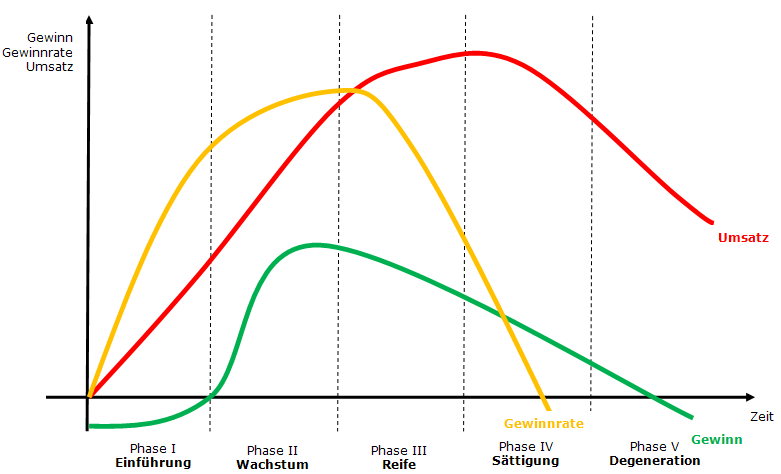
\includegraphics[width=0.6\textwidth]{BilderAllgemein/produktlebenszyklus.png}
	\caption{Einzelnen Phasen des Produktlebenszyklus \cite{Deef09}}
	\label{img:produktlebenszyklus}
\end{figure}

Bei international vermarkteten Produkten kann es vorkommen, dass sich die Produkte abhängig von der Region in unterschiedlichen Phasen befinden. Weiters stellt der Produktlebenszyklus keine genaue Prognose für jedes Produkt dar und kann somit variieren. Im Folgenden werden die einzelnen Phasen beschrieben \cite{Poeschek00}.

\textbf{Einführungsphase}

In der ersten Phase ist der Umsatz noch sehr gering und der Gewinn negativ, da das Produkt erst am Markt eingeführt wurde und hohe Einführungskosten vorhanden sind. Eine steigende Tendenz ist jedoch schon ersichtlich. Gute Werbung und Öffentlichkeitsarbeit sind in dieser Phase unerlässlich und können mitentscheiden, ob das Produkt den Einstieg schafft oder zum Flop wird. Bei Erreichen des Break Even Points ist die Einführungsphase beendet und die Wachstumsphase beginnt \cite{Poeschek00}.

\textbf{Wachstumsphase}

In der Wachstumsphase wurde das Produkt erfolgreich am Markt eingeführt und Umsatz und Absatz steigen stark an. Marktanteile wachsen und Konkurrenten werden auf das Produkt aufmerksam. Es gilt durch Unterstützung von Marketingaktivitäten den Markt mit dem eigenen Produkt weiter zu durchdringen. Weiters sollten in dieser Phase die Herstellungskosten durch das Mengenwachstum gesenkt werden \cite{Poeschek00}.

\textbf{Reifephase}

In der Reifephase hat sich das Produkt so weit am Markt verbreitet, dass das Wachstum stagniert. Sie gilt allgemein als die längste und profitabelste Phase und sollte deshalb so weit als möglich gestreckt werden. Die Verteidigung der Marktposition gegenüber den Konkurrenten ist essentiell. Der Übergang in die Reifephase kann an mehreren Faktoren erkannt werden. Dazu gehört die Zunahme der internationalen Konkurrenz, der Kampf um Marktanteile sowie die Zunahme von Preis- und Serviceorientierung aufgrund der wachsenden Erfahrungen der Unternehmen. Weiters erreicht der Gewinn in dieser Phase seinen Höhepunkt und beginnt wieder zu sinken, wohingegen der Umsatz weiter steigt \cite{Poeschek00}.

\textbf{Sättigungsphase}

Die Sättigungsphase ist dann erreicht, wenn keine zusätzlichen Marktteilnehmer mehr gewonnen werden können. Wie in Abb. \ref{img:saettigung} ersichtlich, muss das Unternehmen an diesem Punkt entscheiden, ob eine Neuorientierung erfolgt, das Produkt aufgegeben wird oder solange weitergeführt wird, wie Gewinne erwirtschaftet werden. Weiters sollten in der Sättigungsphase die Ursachen für den Rückgang der Nachfrage untersucht werden \cite{Poeschek00}.

\begin{figure}[h!]
	\centering
	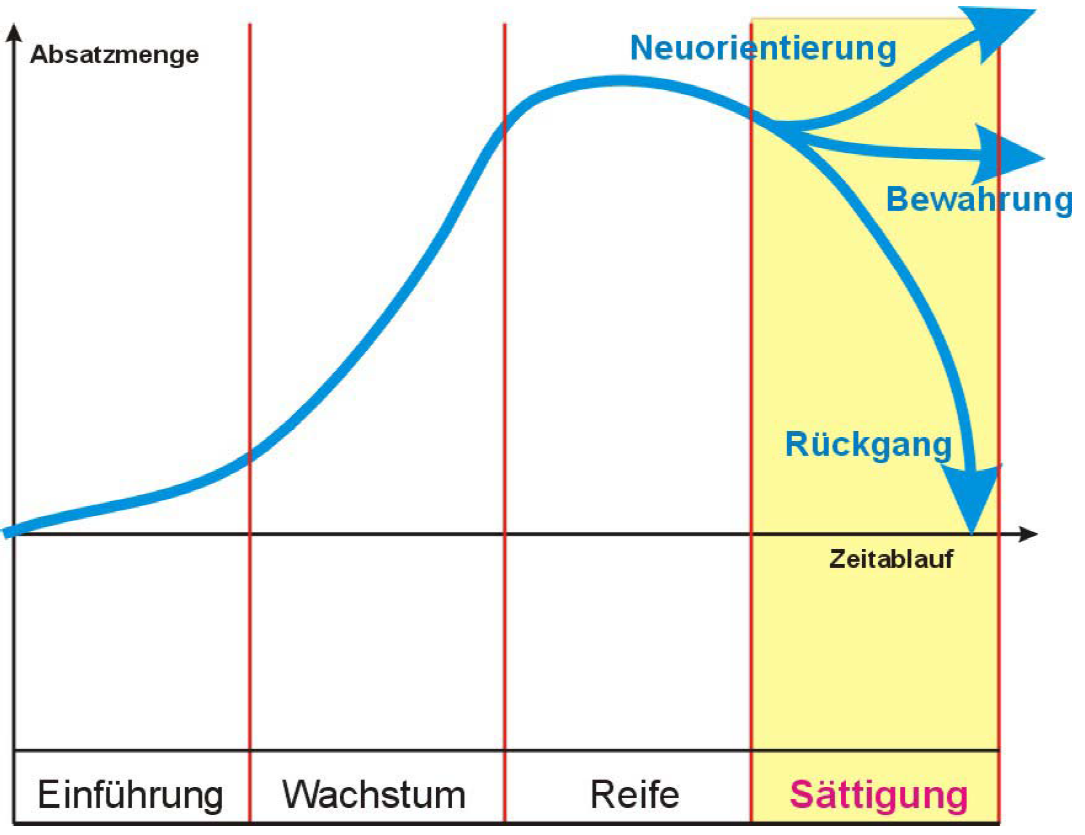
\includegraphics[width=0.45\textwidth]{BilderAllgemein/saettigung.png}
	\caption{Sättigungsphase Entscheidungen \cite{Poeschek00}}
	\label{img:saettigung}
\end{figure}

\textbf{Rückgangsphase}

In der Degeneration beziehungsweise Rückgangsphase schrumpft der Absatzmarkt kontinuierlich und dem Umsatzrückgang kann auch durch gezielte Marketingmaßnahmen nicht entgegengewirkt werden. Wenn vom Unternehmen in der Sättigungsphase keine Neuorientierung erfolgt, ist das Produkt mit Ende dieser Phase "gestorben" \cite{Poeschek00}.

\subsection{Technologielebenszyklus}

Das Modell des Technologielebenszyklus ist Teil des strategischen Innovationsmanagements und dient dazu, die Position einer Technologie in ihrem jeweiligen Lebenszyklus zu finden. Es wird davon ausgegangen, dass der von der Technologie durchlaufene Zyklus von der Nachfrage nach Produkten und Services, welche auf dieser Technologie beruhen, abhängt \cite{Bru06} \cite{Schumann03}.

Im Allgemeinen ist der Technologielebenszyklus ein an den Produktlebenszyklus angepasster idealtypischer Entwicklungsverlauf einer Technologie. Wie in Abb. \ref{img:technologielebenszyklusmodell} ersichtlich ist der Kurvenverlauf s-förmig und kann in die vier Technologiephasen \textbf{Entstehung, Wachstum, Reife und Alter} unterteilt werden \cite{Schumann03}.

\begin{figure}[h!]
	\centering
	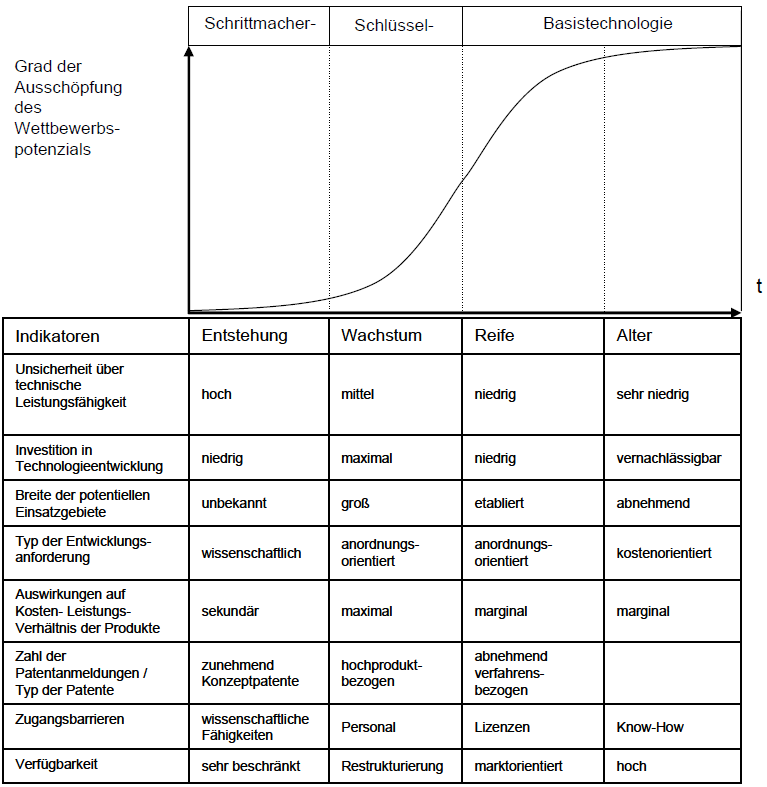
\includegraphics[width=0.8\textwidth]{BilderAllgemein/technologielebenszyklusmodell.PNG}
	\caption{Technologielebenszyklusmodell von Arthur D. Little \cite{Gerpott05}}
	\label{img:technologielebenszyklusmodell}
\end{figure}

Weiters werden drei Technologietypen unterschieden, welche als Schrittmacher- Schlüssel- und Basistechnologie bekannt sind \cite{Schumann03}.

\textbf{Schrittmachertechnologien} sind soeben erst am Markt eingeführt worden und befinden sich am Anfang ihrer Entwicklung. Mit zunehmender Verbreitung werden sie zu Schlüsseltechnologien heranreifen, sofern sie nicht zuvor vom Markt verdrängt werden. \\
Hat die Technologie eine Marktreife erreicht, so wird von \textbf{Schlüsseltechnologien} gesprochen. In dieser Phase existiert noch ein erhebliches Verbesserungspotential und die Möglichkeit für den Aufbau von Wettbewerbsvorteilen. \\
Ab einer gewissen Reife spricht man von \textbf{Basistechnologien}. Aufgrund einer meist bereits großen allgemeinen Verfügbarkeit ist das wettbewerbsstrategische Potential in dieser Phase sehr gering \cite{Bru06} \cite{Schumann03}.

\subsubsection{S-Kurve}

Zum Vergleichen zweier Technologien in Bezug auf ihre Vorteilhaftigkeit wird das Konzept der \textbf{S-Kurve}, siehe Abb. \ref{img:s-kurve}, verwendet \cite{Schumann03}.

\begin{figure}[h!]
	\centering
	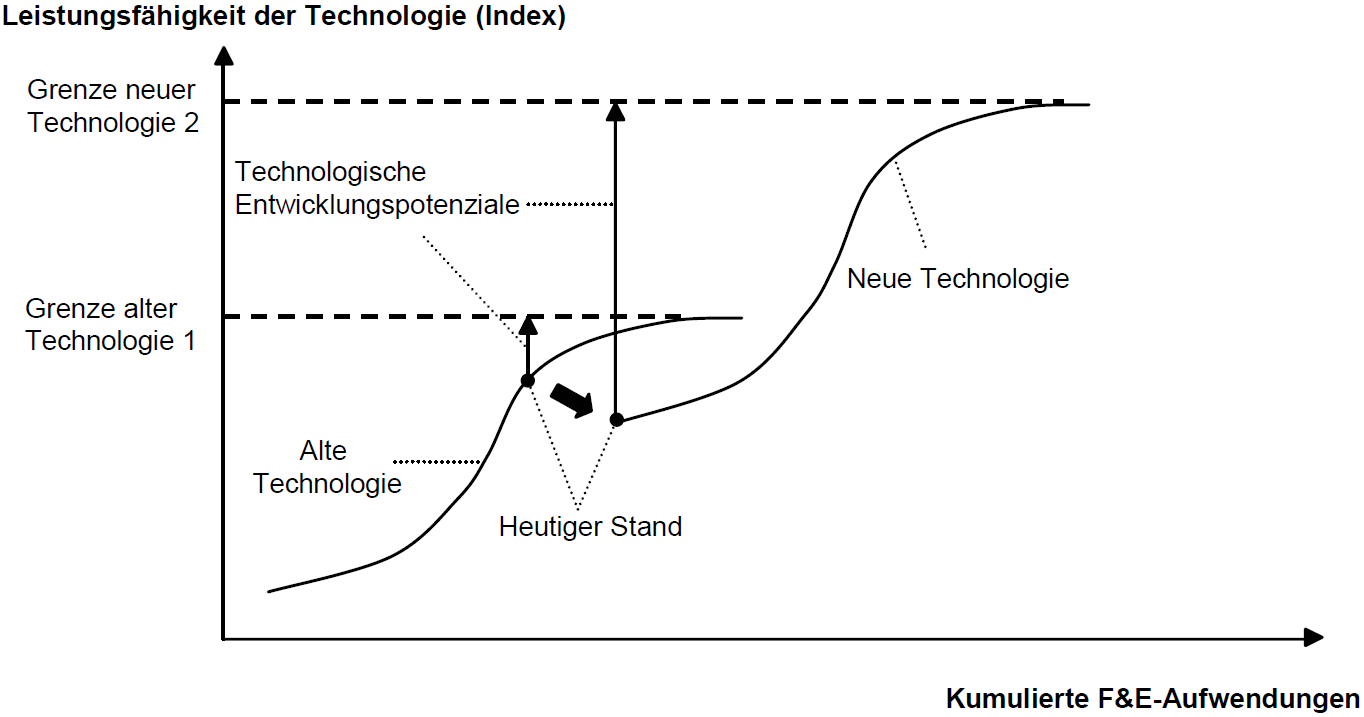
\includegraphics[width=0.9\textwidth]{BilderAllgemein/s-kurve.PNG}
	\caption{S-Kurven Modell von McKinsey \cite{Gerpott05}}
	\label{img:s-kurve}
\end{figure}

Zu Beginn lässt sich die Leistungsfähigkeit mit relativ geringen Investitionen steigern. Mit zunehmender Reife wird das Beibehalten des Leistungszuwachses immer schwerer, wodurch sich ein Wechsel zu einer Technologie mit höherer Leistungsfähigkeit empfiehlt. Die Grenze einer Technologie wird oft durch natürliche Eigenschaften, wie Größe oder Materialeigenschaften, welche nicht mehr gesteigert werden können, bestimmt \cite{Bru06}.

Das Konzept der S-Kurve wurde von FOSTER entwickelt, welcher das Erstellen in vier Schritte unterteilt \cite{Foster86}:

a) Identifikation der Alternativen

Eine Technologie dient als Lösung eines spezifischen Problems. Um dieses Problem zu lösen wird zu Beginn der Entwicklung einer Technologie ein Problemlösungsvorgehen erstellt. Im ersten Schritt des Aufstellens einer S-Kurve werden Alternativen zum bereits existierenden Problemlösungsvorgehen identifiziert und die jeweiligen Möglichkeiten notiert \cite{Bru06}. 

b) Identifikation relevanter Leistungsparameter

Im zweiten Schritt gilt es, den Markt beziehungsweise die Nutzer in Produktnutzergruppen zu unterteilen um im nächsten Schritt die Ansprüche an das Produkt identifizieren zu können. Für jede dieser Produktnutzergruppen werden Leistungsparameter definiert, welche so nah als möglich in Verbindung mit den Charakteristika des gewählten technischen Lösungsansatzes stehen sollten. Es gilt zu beachten, dass sich die Leistungsparameter im Laufe der Zeit ändern können. Vergangenheitsdaten dürfen jedoch als Anhaltspunkt verwendet werden \cite{Bru06}.

c) Kalkulation technologischer Leistungsgrenzen

In diesem Schritt werden die Grenzen für jeden der zuvor definierten Leistungsparameter kalkuliert. Dabei wird die zugrunde liegende Technologie genauer untersucht. Zur Unterstützung der Kalkulation kann zum Beispiel auf technisches Fachpersonal des Unternehmens zurückgegriffen werden. Wichtig ist eine numerische Festlegung der Leistungsgrenzen. Dieser Schritt ist für die Praxis enorm wichtig, da das technologische Entwicklungspotential der Technologie aus der Differenz zwischen dem errechneten Limit und dem aktuellen Technologiestand bestimmt werden kann \cite{Bru06}.

d) Grafische Darstellung der S-Kurve

Der letzte Schritt befasst sich mit der grafischen Umsetzung, welche meist durch einen mathematischen Ansatz ermöglicht wird. Als Beispiel hierfür dient Abb. \ref{img:s-kurve}. Zuerst werden die historischen Daten, bestehend aus der Leistungsperformanz der Technologie sowie den aufsummierten \acp{FE} Investitionen kalkuliert und dargestellt. Die Grenzen der Technologie werden als horizontale Linien gezeichnet. Die Kurve selbst kann durch drei Punkte vollständig bestimmt werden. Mit zwei historischen Datenpunkten, dem Limit und den dafür notwendigen \ac{FE} Investitionen wird die Kurve berechnet und aufgetragen \cite{Bru06}.

Schwierig gestaltet sich in der Praxis das Einschätzen der \ac{FE} Investitionen einer noch nicht vorhandenen Technologie \cite{Bru06}.
%% Eventuell noch über Probleme der S-Kurve sprechen

\subsection{Lebenszykluskonzepte in dieser Arbeit}

Die Erläuterung der Lebenszyklusmodelle soll aufzeigen, dass sich Technologien stets weiterentwickeln beziehungsweise eine Technologie am Ende ihres Zyklus von einer neueren Technologie abgelöst wird. Die Verbreitung solcher Technologien ist jedoch sehr stark von Branche und Region abhängig. Ein Beispiel hierfür ist, dass in Europa das Bedürfnis nach Transportmitteln erfüllt ist, während es sich in vielen Regionen Asiens erst in der Einführungs- beziehungsweise Wachstumsphase befindet \cite{Bru06}. 

Wird als weiteres Beispiel Rechenleistung verwendet, so befindet sich Europa noch in der Wachstumsphase, während es in Bhutan bis vor einigen Jahren noch gar kein Bedürfnis nach Rechenleistung gab. 

\section{IT Kennzahlen}

IT Kennzahlen dienen als Maßgrößen für IT relevante Aspekte sowie zur Ermittlung von Abweichungen zwischen dem Soll- und Istwert. Sie geben einen schnellen Überblick über die Kosteneffizienz der gesamten IT-Infrastruktur und bieten somit einen Vergleich zum Wettbewerb. IT Kennzahlen dienen als Informationsquelle und als Steuerungselement für IT Projekte und Ressourcen \cite{Gadatsch10}. 

\begin{figure}[h!]
	\centering
	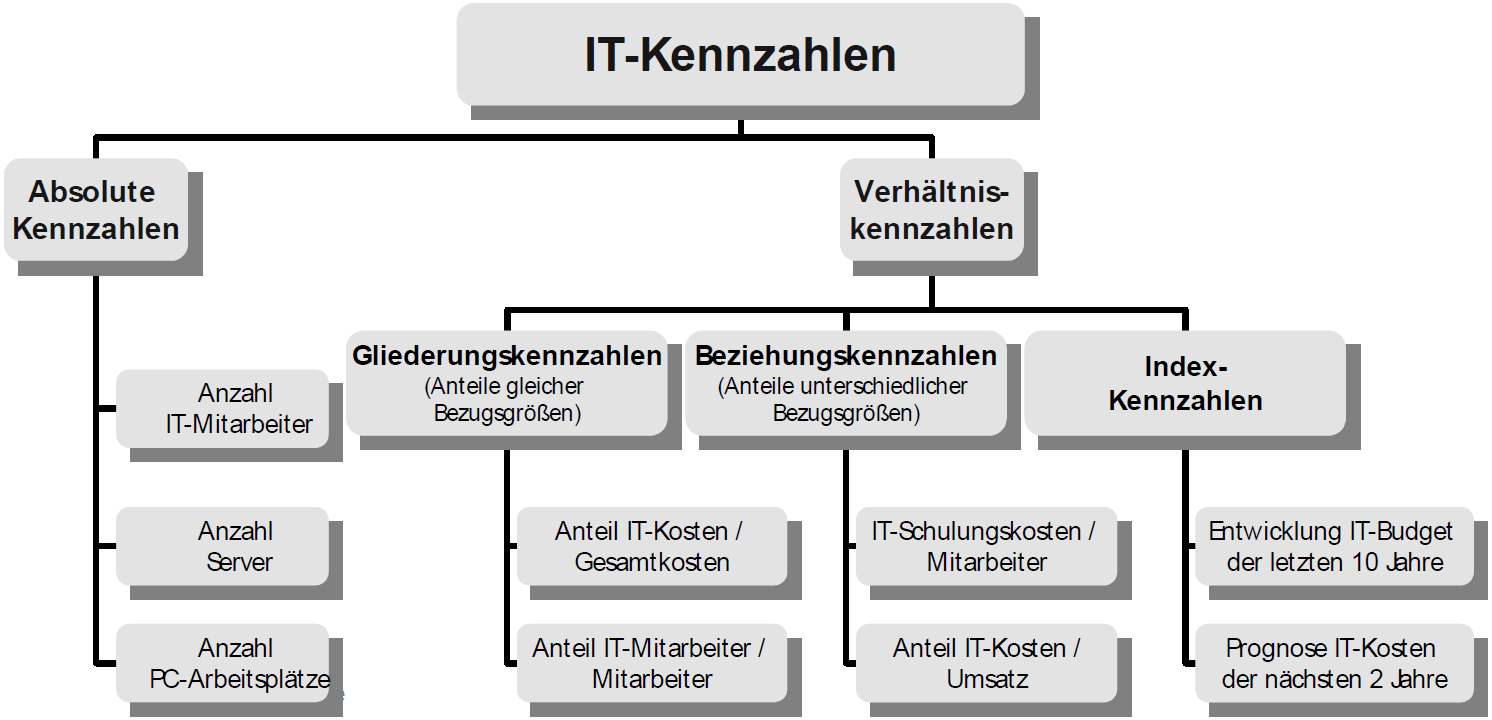
\includegraphics[width=0.8\textwidth]{BilderAllgemein/it_kennzahlen.PNG}
	\caption{Übersicht IT Kennzahlen \cite{Gadatsch10}}
	\label{img:uebersicht_it_kennzahlen}
\end{figure}

Abb. \ref{img:uebersicht_it_kennzahlen} zeigt die Struktur von IT Kennzahlen, welche sich in absolute Kennzahlen und Verhältniskennzahlen aufteilen. Verhältniskennzahlen splitten sich wiederum in Gliederungskennzahlen, Beziehungskennzahlen und Indexkennzahlen. \\
Im Vergleich zu den absoluten Kennzahlen, welche bereits aus messbaren, numerischen Größen bestehen, wird bei den Verhältniskennzahlen der Wert durch Berechnung ermittelt. \\
Bei den Gliederungskennzahlen wird eine Teilgröße in Beziehung zu einer Gesamtgröße gesetzt. Ein Beispiel ist der Anteil an IT-Kosten im Vergleich zu den Gesamtkosten. \\
Die Beziehungskennzahl gilt als aussagekräftigste Kennzahl. Für die Berechnung werden Größen, welche in einem sachlogischen Zusammenhang stehen, in Verbindung gesetzt. Als Beispiel dienen die IT-Schulungskosten / Mitarbeiter. \\
Indexkennzahlen werden verwendet, um eine zeitliche Veränderung von gleichartigen Kennzahlen darzustellen. Für die Berechnung wird ein Basiswert zu einem Basiszeitpunkt gleich 100 gesetzt. Eine zu einem späteren Zeitpunkt erfasste Größe stellt dann die Entwicklung als Vergleichswert dar. Die Prognose der IT-Kosten für die nächsten zwei Jahre ist ein Beispiel der Indexkennzahlen \cite{Gadatsch10} \cite{Jung07}.

Die folgende Liste zählt die wichtigsten Analysebereiche für IT Kennzahlen inklusive Beispielen für die jeweiligen Bereiche auf:

\begin{itemize}[noitemsep]
\item Wirtschaftlichkeit $\rightarrow$ Welche Vorteile bringt die Durchführung eines IT Projektes? Welche Kosten sind damit verbunden? Werden Gewinne erzielt? Wird der Bekanntheitsgrad des Unternehmens gesteigert?
\item Innovationsgrad der IT $\rightarrow$ Lohnt sich ein Upgrade der IT Hardware? Soll die veraltete IT Hardware weiter betrieben werden?
\item Prozessqualität $\rightarrow$ Welchen Einfluss hat die IT auf den Geschäftsprozess? 
\item Ressourcenauslastung in der IT $\rightarrow$ Welche Ausbildung haben die IT Mitarbeiter? Ist die Nutzung der Mitarbeiter effizient? Wie viele IT Mitarbeiter sind aktiv \cite{Gadatsch10}?
\end{itemize}

\subsection{IT-Kennzahlensysteme}

Aufgrund der geringen Aussagekraft von einzelnen, isolierten IT Kennzahlen werden im IT Management IT-Kennzahlensysteme verwendet. Diese Kennzahlensysteme stellen einzelne IT Kennzahlen in einen logischen Zusammenhang und unterstützen somit ein fachgerechtes IT Controlling \cite{Gadatsch10}. 

Es existieren mehrere IT-Kennzahlensysteme, welche im Laufe der Zeit von unterschiedlichen Firmen entwickelt wurden. \\
Das SVD-Kennzahlensystem, entwickelt 1980 von der Schweizerischen Vereinigung für Datenverarbeitung, ist hauptsächlich auf die Planung, Kontrolle und Steuerung der Wirtschaftlichkeit von IT-Systemen ausgelegt. Im Speziellen wird hierzu das Management, der Benutzer und die Informationsverarbeitung berücksichtigt \cite{Gadatsch10}.

\begin{figure}[h!]
	\centering
	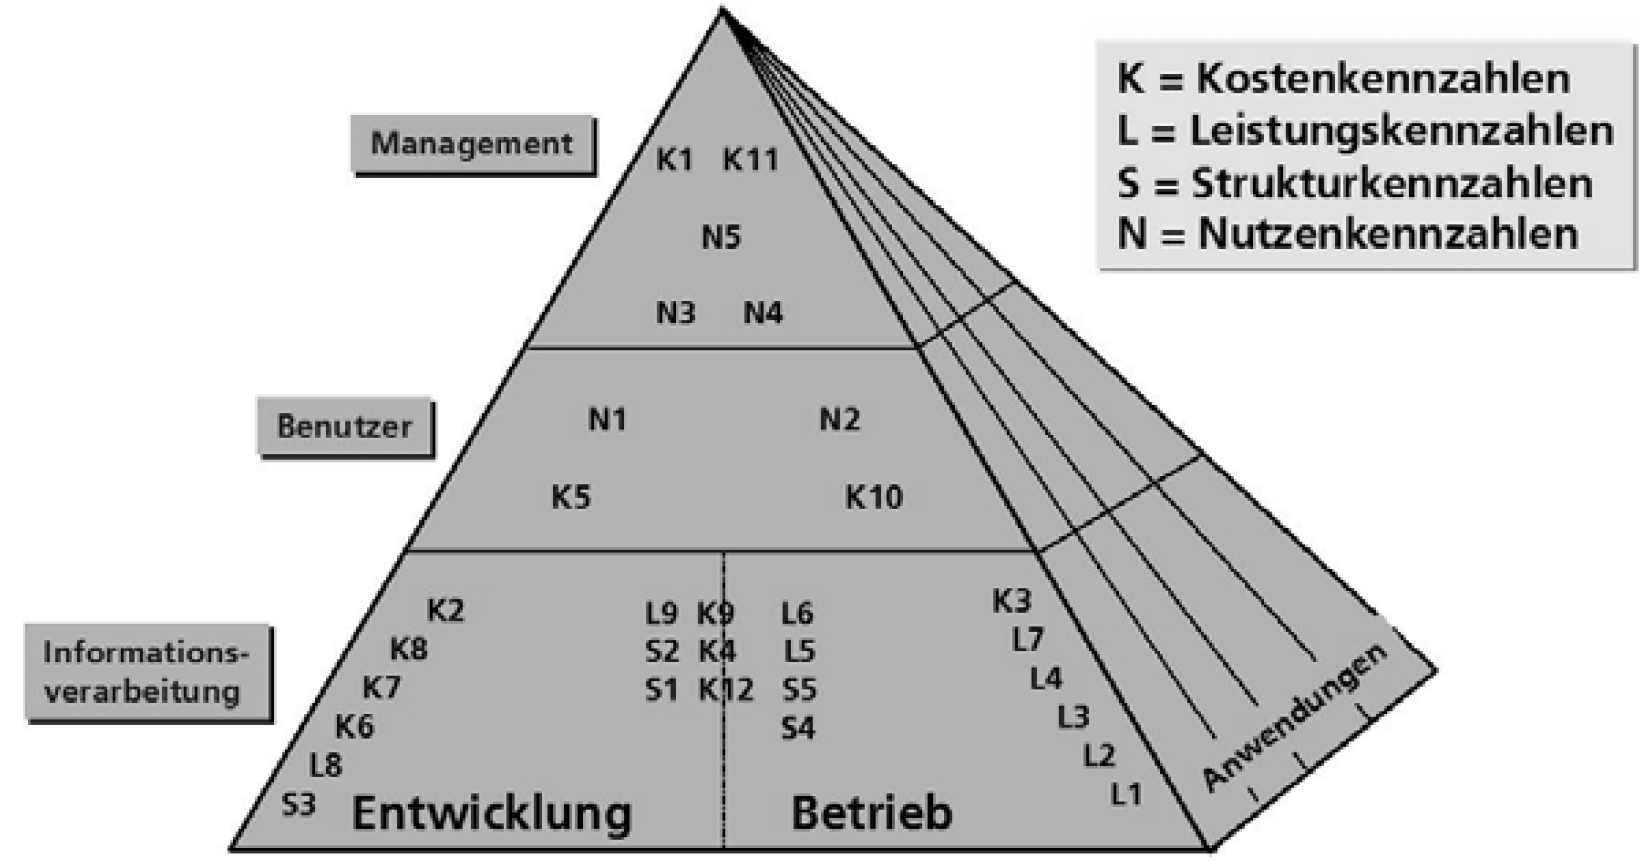
\includegraphics[width=0.8\textwidth]{BilderAllgemein/svd_kennzahlensystem.PNG}
	\caption{SVD Kennzahlensystem \cite{Biethahn00}}
	\label{img:svd_kennzahlensystem}
\end{figure}

Abb. \ref{img:svd_kennzahlensystem} zeigt das SVD Kennzahlensystem. Es besteht aus 30 Kennzahlen, welche sich in die vier Gruppen Leistungs-, Kosten-, Struktur- und Nutzenkennzahlen unterteilen. Die Leistungs-, Kosten- und Strukturkennzahlen lassen sich aus dem internen Rechnungswesen und der Personalwirtschaft generieren. Die Nutzenkennzahlen geben an, wie sinnvoll die Nutzung der IT im Vergleich zu keiner Nutzung der IT ist \cite{Gadatsch10}.

Im folgenden sind drei Kennzahlen ersichtlich, welche speziell im Rahmen dieser Bachelorarbeit relevant sind \cite{Gadatsch10}:

\textbf{L1 - Verfügbarkeit:}

$$Verfügbarkeit = \frac{Sollstunden - Ausfallstunden}{Sollstunden}$$

Die Verfügbarkeit definiert die Wahrscheinlichkeit, dass ein Objekt (Komponente oder System) zu einem bestimmten Zeitpunkt eine bestimmte Leistung erbringt. Sie wird in mehrere Klassen unterteilt, wobei zwischen einfacher Verfügbarkeit mit 99,5\%, Hochverfügbarkeit mit 99,999\% und Non-Stop Verfügbarkeit mit 100\% unterschieden wird. Um einen Ausfall zu verhindern gilt es Datenverarbeitungssysteme und Kommunikationswege stets redundant auszuführen \cite{Availability}.

Unter Anbetracht der obigen Formel, umgeändert auf Minuten, bedeutet eine Hochverfügbarkeit eine erlaubte Ausfallzeit von 5,256 Minuten in einem Zeitraum von einem Jahr: 

$Ausfallzeit = Sollzeit - (Verfügbarkeit * Sollzeit) = (365 * 24 * 60) - (0.99999 * 365 * 24 * 60) = 5,256$

\textbf{L2 - Zuverlässigkeit:}

$$Zuverlässigkeit = \frac{Sollstunden}{Anzahl\;der\;Ausfälle}$$

Die Zuverlässigkeit beschreibt die Wahrscheinlichkeit, ein Objekt zu einem bestimmten Zeitpunkt in einem funktionierenden Zustand vorzufinden. Die mittlere Zeit \ac{MTBF}, welche zwischen zwei Fehlern eines Objektes vergeht, wird als Maß der Zuverlässigkeit bezeichnet. \\
Je länger diese Zeit ist, desto zuverlässiger ist das Objekt. In der Theorie kann diese Zeit gegen unendlich gehen, in der Praxis jedoch nicht, da die Zeit durch die Lebensdauer begrenzt ist. Mit zunehmender \ac{MTBF} nimmt jedoch die Anzahl an Fehlern innerhalb eines definierten Zeitraums ab \cite{Eberlin14}. 

\begin{figure}[h!]
	\centering
	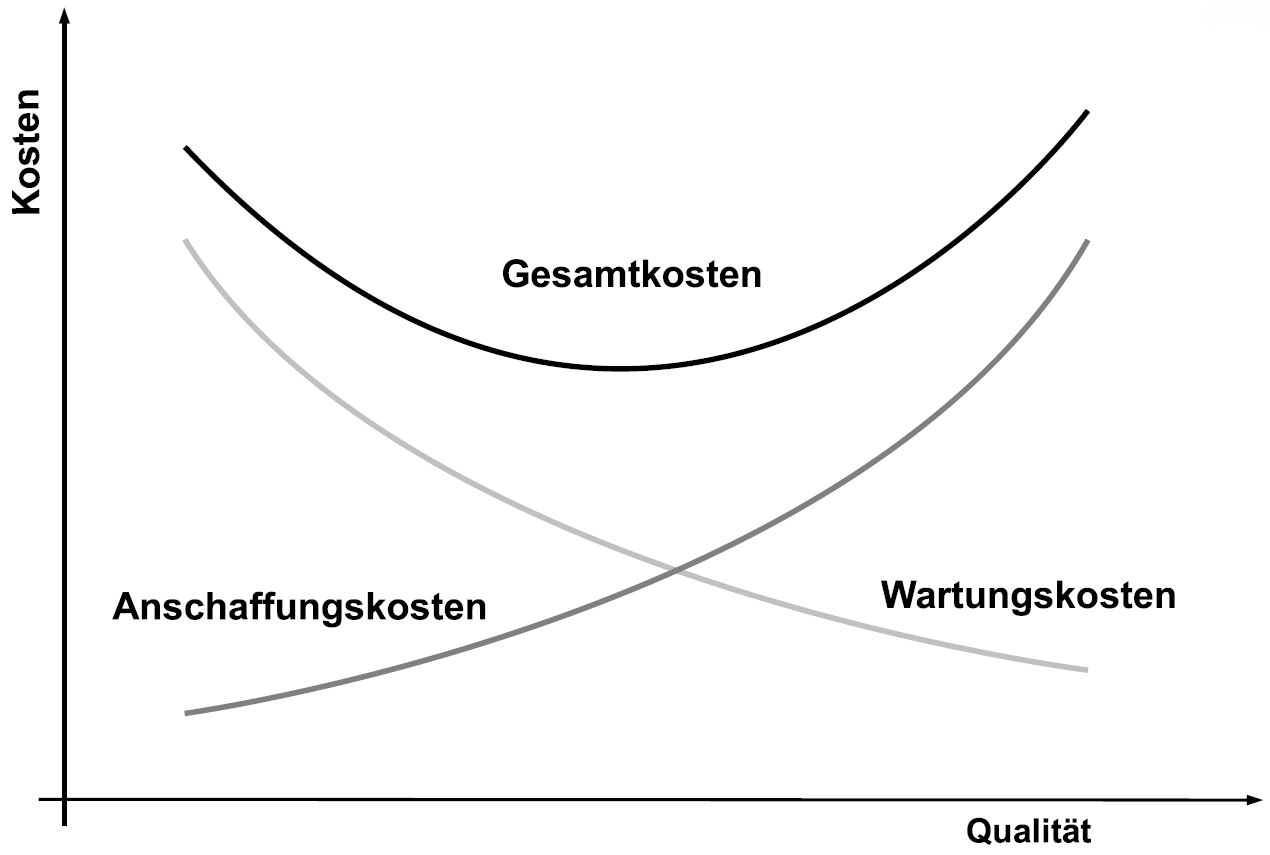
\includegraphics[width=0.6\textwidth]{BilderAllgemein/kosten_der_zuverlaessigkeit.PNG}
	\caption{Kosten der Zuverlässigkeit \cite{Eberlin14}}
	\label{img:kosten_der_zuverlaessigkeit}
\end{figure}

Abb. \ref{img:kosten_der_zuverlaessigkeit} zeigt einen typischen Verlauf von Anschaffungskosten, Wartungskosten und den daraus resultierenden Gesamtkosten. Die Kosten der Zuverlässigkeit sind beim Schnittpunkt zwischen Anschaffungskosten und Gesamtkosten minimal. Es gilt somit, Kosten und Qualität gegeneinander abzuwägen um Gesamtkosten zu sparen \cite{Eberlin14}.

\textbf{L3 - Durchschnittliche Reparaturzeit:}

$$Durchschnittliche\;Reperaturzeit = \frac{Reparaturzeit}{Anzahl\;von\;Reparaturen}$$

Die durchschnittliche Reparaturzeit ist Teil der Instandhaltbarkeit. Sie gibt an, wie schnell und mit welchem Aufwand ein Objekt nach einem Fehler wieder in den operativen Zustand gebracht werden kann \cite{Maintainability}.

Laut DIN IEC 60300-3-10 ist die Instandhaltbarkeit folgendermaßen definiert:

\begin{quote}
Fähigkeit einer Einheit, unter gegebenen Anwendungsbedingungen in einem Zustand erhalten bzw. in ihn zurückversetzt werden zu können, in dem sie eine geforderte Funktion erfüllen kann, wobei vorausgesetzt wird, dass die Instandhaltung unter den gegebenen Bedingungen mit den vorgeschriebenen Verfahren und Hilfsmitteln durchgeführt wird. \upshape \cite[S. 9]{Din04}.
\end{quote}

\clearpage
%\pagenumbering{arabic}
\chapter{Selection of used technologies}

\thispagestyle{standard}
\pagestyle{standard}

\section{Layer 2 versus Layer 3 device}

Before explaining \acp{VLAN} in detail, it is important to understand the concept of switches. A network switch is used to connect several devices together on a computer network. When speaking about the functionality "switching", a Layer 2 device of the \ac{OSI} model is meant. When performing "switching" the switch uses hardware addresses, in particular the \ac{MAC} address, to forward data from one port to another. \\
Some switches, also known as Multilayer Switches or Layer 3 switches, support "routing functionality", thus referring to a Layer 3 device of the \ac{OSI} model. A Layer 3 device uses \ac{IP} addresses to perform packet forwarding. The most widely known L3 device is the router \cite{wiki:switch}. 

Switches with Layer 2 functionality are used to connect same subnets to each other. In order to enable data communication between different IP subnets, a Layer 3 device with routing functionality is needed! 
Moreover it is important to know, that L2 switches, on the contrary to routers, do not separate broadcast domains. This means, that broadcast messages sent by a client do not traverse a router by default \cite{wiki:switch}.

\section{VLANs}

A \ac{VLAN} is used to allow data communication for a group of devices (e.g. computer, server, firewall and more) as if they were attached to the same wire, although in reality they can be connected to totally different LAN segments (e.g. one device is located in building A and the other device in building B on the other side of the street). \\
Most of the time \acp{VLAN} are associated with \ac{IP} subnets. A \ac{VLAN} defines an own broadcast domain in a Layer 2 network. \acp{VLAN} are typically defined at switches and are based on logical instead of physical connections. \\
Figure \ref{img:example_of_vlans} shows three different \acp{VLAN} that span multiple floors \cite{cisco:vlan}. 

\begin{figure}[ht!]
	\centering
	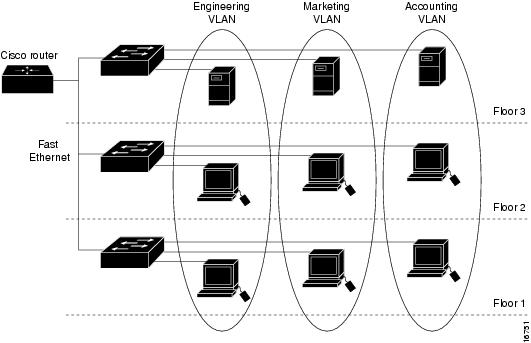
\includegraphics[width=0.9\textwidth]{BilderAllgemein/example_vlans.jpg}
	\caption{Example of VLANs \cite{cisco:vlan}}
	\label{img:example_of_vlans}
\end{figure}

\subsection{Trunks and tagged VLANs}

Trunk links are required to pass several VLANs from one switch to another when using only one logical connection. On a Cisco switch a port can be configured for either access or trunk mode. Access ports belong to only one VLAN and frames exiting such a port are not tagged (marked). Trunk ports on the other way allow the transmission of several VLANs. In order to be able to distinguish the VLAN origin of the frame it is marked with a VLAN tag. This marking procedure is called tagging and uses some tagging mechanism (ISL or 802.1Q, whereby 802.1Q is the most commonly used). \\
A tagged and untagged frame mainly distinguishes between having a VLAN tag or not.

Fig. \ref{img:ethernet_ii_frame} shows the concept of tagging by looking at the most common Ethernet frame type Ethernet-II (IEEE 802.3) including an inserted 802.1Q VLAN tag \cite{ciscopress:vlan}.

\begin{figure}[ht!]
	\centering
	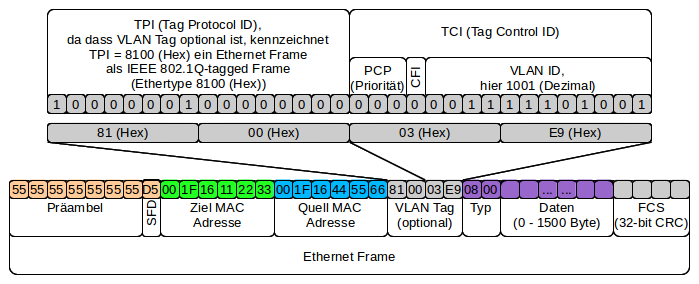
\includegraphics[width=1\textwidth]{BilderAllgemein/vlan_tag.png}
	\caption{Ethernet-II frame with 802.1Q VLAN tag \cite{krenn:tag}}
	\label{img:ethernet_ii_frame}
\end{figure}

\newpage
\textbf{Native VLAN}

The only VLAN that is not tagged on a trunk is called the native VLAN. This means that all packets belonging to the native VLAN do not have a VLAN tag. When configuring a trunk on a Cisco switch and not specifically defining a native VLAN, the native VLAN will be VLAN 1.

\section{Hypervisor}

A hypervisor is a piece of software that allows for one physical device (e.g. computer or server) to share its resources amongst several \acp{VM} running on that physical device. \\
Speaking of terminology, the server that is running the hypervisor is called host machine and the VMs are called guest machines. As displayed in fig. \ref{img:type_1_type_2_hypervisor} the hypervisors are divided into Type-1 (native or bare-metal) hypervisors and Type-2 (hosted) hypervisors \cite{bill:hypervisor}.

\begin{figure}[ht!]
	\centering
	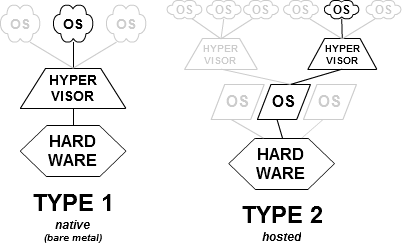
\includegraphics[width=0.8\textwidth]{BilderAllgemein/hypervisor.png}
	\caption{Difference between Type-1 and Type-2 hypervisor \cite{wiki:hypervisor}}
	\label{img:type_1_type_2_hypervisor}
\end{figure}

\textbf{Type-1 Hypervisor}

When installing this type, the hypervisor is directly installed as an operating system. A huge advantage is, that the hypervisor can directly communicate with the underlying physical hardware. These physical hardware resources are then \textit{paravirtualized} and provided to the virtual machines. This type of hypervisor is the preferred method for productive server environments. One hypervisor of this type is VMware ESXi, which has also been used within the IT infrastructure at RITH \cite{bill:hypervisor}.

\textbf{Type-2 Hypervisor}

When speaking of this type, a hypervisor that can be directly installed on an operating system is meant. Two popular freeware products are VMware Player and Oracle VM VirtualBox. These types of hypervisor are not used for productive server environments. They are more used to quickly do some tests and experiments without crashing the own operating system \cite{bill:hypervisor}. 

An example would be that someone would like to test a linux operating system. He/she then installs a Type-2 Hypervisor on his/her operating system (e.g. Windows 10) and creates a VM for Linux. After that he/she is able to do everything within this VM without affecting his/her used operating system Windows 7.

\textbf{Paravirtualization Tools}

These tools (in case of VMware also called VMware Tools) are installed on the VMs to perfectly support the paravirtualized hardware, that is provided by the hypervisor \cite{bill:hypervisor}. 

The following shows an example regarding the Paravirtualization Tools. \\
The hypervisor is accessing the \ac{NIC} of the physical server and paravirtualizing it, in order to provide this specific \ac{NIC} to several VMs. When creating the VM, this paravirtualized \ac{NIC} is then chosen as the network card for the VM. To get optimal performance, the Paravirtualization Tools provide a specific driver for this paravirtualized \ac{NIC}, that can be installed on the OS of the guest machine.

\chapter{IT Infrastructure}

\thispagestyle{standard}
\pagestyle{standard}

\section{Final Hardware}

Regarding the hardware constellation of the main server and the backup server it was important to have a \ac{RAID} controller available in order to obtain reliability. 

\textbf{Storage space design:}

The \acp{HDD} on the main server have been configured to operate in a \ac{RAID} 5. When speaking of \ac{RAID} 5, there always is one \ac{HDD} used for parity purposes, whereby the usable capacity is then reduced by the size of one \ac{HDD}. Furthermore, when configuring a \ac{RAID} 5, every \ac{HDD} has to be the same size. The main server has four 1.2 TB \acp{HDD}. This results in a net capacity (usable capacity) of 3.6 TB. 

The \ac{NAS} has two 6 TB \acp{HDD} and is configured in a \ac{RAID} 1. This type of \ac{RAID} performs a mirroring of hard disks, what means that one \ac{HDD} can be damaged and the data is still available. Due to the RAID 1 the net capacity of the \ac{NAS} results in 6 TB. \\
The backup server is also configured in a \ac{RAID} 5. Based on the five \acp{HDD} with a size of 300 GB each the net capacity is 1.2 TB. \\
Table \ref{tbl:net_capacity_of_components} summarizes the calculations explained above.
\vspace{10pt}

\begin{table}[ht!]
\centering
\begin{tabular}{C{3cm}|C{2cm}|C{5cm}}
\textbf{Component} & \textbf{RAID} & \textbf{Net capacity} \\
\hline
Main Server & 5 & 3.2 TB \\
\hline
Backup Server & 5 & 1.2 TB \\
\hline
NAS & 1 & 6 TB \\
\end{tabular} 
\caption{Net capacity of components}
\label{tbl:net_capacity_of_components}
\end{table}

The limiting component regarding the storage space was the local storage of the backup server. Due to this reason the decision was made to store the backup files on the \ac{NAS}. The backup server only hosts the operating system on the local storage and the actual backup files are accessed from the NAS via the \ac{iSCSI} protocol.

Table \ref{tbl:auflistung_finaler_hardware} shows the hardware components that have been installed at \ac{RITH}.

\begin{table}[ht!]
\centering
\begin{tabular}{C{3cm}|C{3cm}|C{5cm}|C{2cm}}
\textbf{Component} & \textbf{Hardware} & \textbf{Specifications} & \textbf{Support} \\
\hline
Main Server & Fujitsu PY TX1320M2/SFF & - Intel Xeon E3-1230v5 \newline - 3x 12GB DDR4-2133 \newline - 4x SAS 12G 1.2TB \newline - RAID 5/6 Controller \newline - 2x 1GbE RJ45 interface & 5 Year On-Site Service \\
\hline
Backup Server & IBM x3650 M3 & - 2x Intel Xeon E5620 @ 2.40GHz \newline - 3x 4GB \newline - 5x SAS 6G 300GB \newline - RAID 5 Controller \newline - 2x 1GbE RJ45 Interface \newline - Redundant power supply & \\
\hline
KVM Switch & Avocent AUTOVIEW 3016 & \\
\hline
Provider Modem & RAD ASMi-52 & \\
\hline
NAS & 1x Synology DS716+ & & \\
\hline
NAS HDDs & 2x Seagate ST6000VN0021 6TB & & \\
\hline
Switch & 4x Cisco SG300-28 & & \\
\hline
Switch & 2x Cisco SG300-52 & & \\
\hline
Access Points & 6x Cisco WAP200 802.11g PoE &  \\
\hline
Access Points & 5x Ubiquiti AC AP Pro & Including \ac{PoE} Injector & \\
\hline
CCTV & 4x Linksys PVC2300 & \\
\hline
CCTV PC & Computer & \\
\hline
Printer & Several & \\
\hline
Computer, Laptops & Several & \\
\end{tabular} 
\caption{Final Hardware}
\label{tbl:auflistung_finaler_hardware}
\end{table}

\section{IT Infrastructure Plan}

\begin{figure}[H]
	\centering
	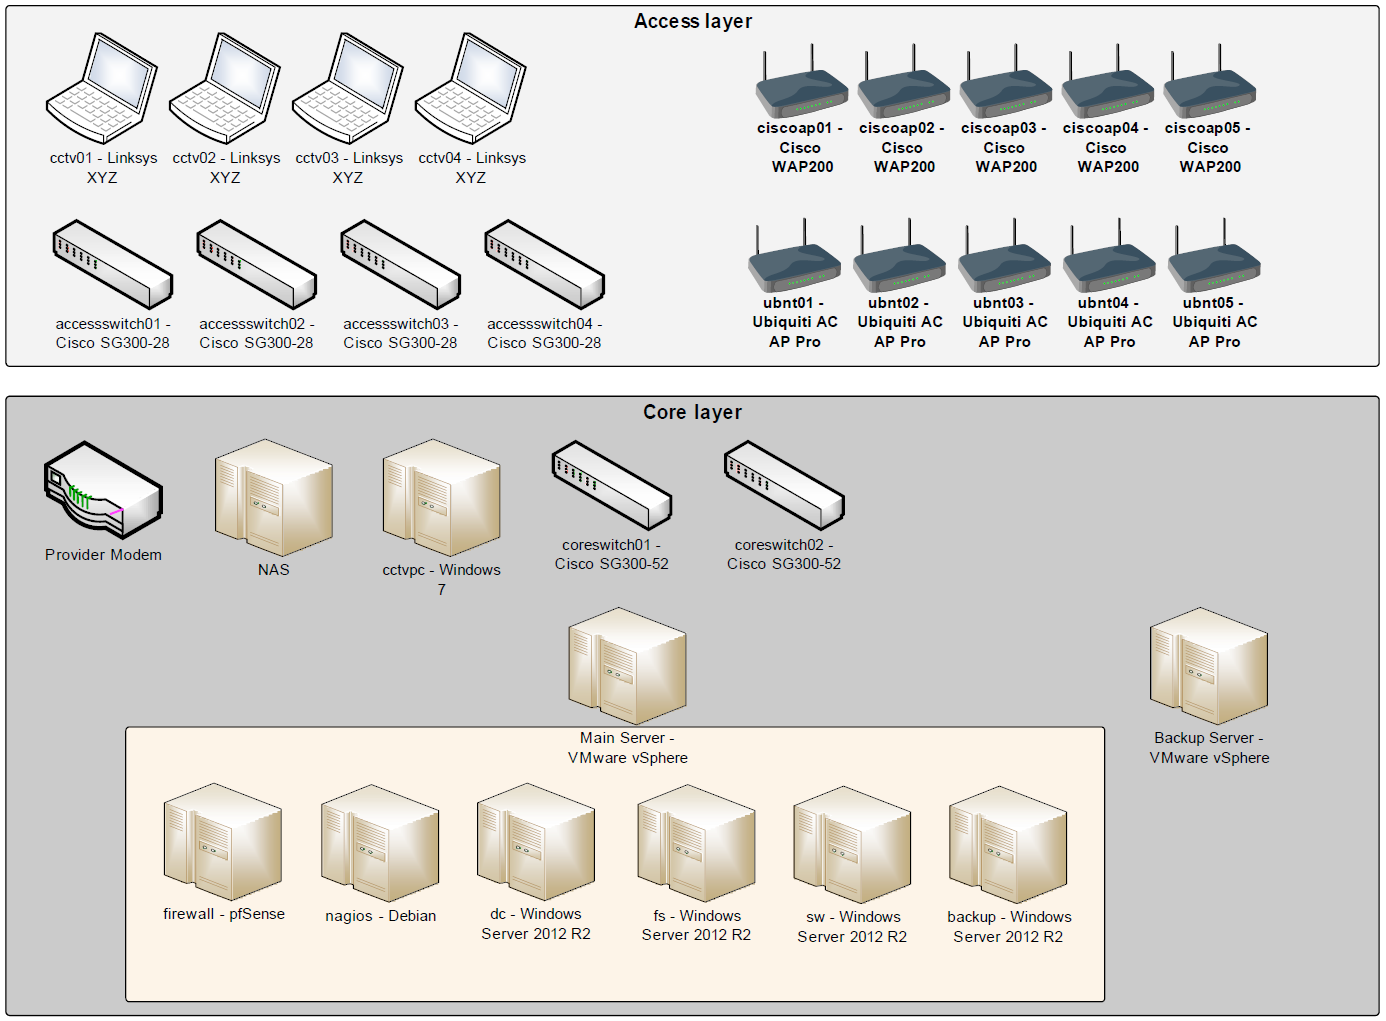
\includegraphics[width=1.0\textwidth]{BilderAllgemein/it_infrastruktur_plan_2.png}
	\caption{IT-Infrastrukturplan}
	\label{img:it_infrastruktur_plan}
\end{figure}

Fig. \ref{img:it_infrastruktur_plan} shows the software and hardware components that were used within the IT infrastructure. It is divided into an access and a core layer. This abstract representation of the IT infrastructure is used to give an overview. Details like \ac{IP} subnets, \ac{IP} addresses, \acp{VLAN}, switch ports or cabling will be shown later.

\subsection{IT Infrastructure Plan in detail}

Core switch 1, as displayed in the plan, establishes the connection between the modem of the \ac{ISP}, the main server, the backup server, the NAS, the CCTV PC, core switch 2 and the remaining access switches. The different IP subnets are separated on the switches by use of VLANs. 

The \ac{OS} of the main server as well as the backup server is VMware vSphere, also called ESXi. Due to this virtualization software, also referred to as hypervisor, several \acp{VM} can be managed on one single physical server. The main server hosts several VMs which are shortly described in the following paragraphs.

On the VM "firewall.ad.rith.edu.bt" the open source operating system pfSense had been installed. This firewall is used to separate and control the traffic between the \ac{WAN} and \ac{LAN} network. Moreover it is used to enable communication between the existing VLANs, which is known as VLAN routing. Monitoring of the WAN bandwidth and WAN quality is also part of the firewall. Therefore the built in graphs called "RRD Graphs", available under Status --> RRD Graphs can be used.

The VM "dc.ad.rith.edu.bt" hosts a Windows Server 2012 R2. This server is used as a domain controller for the local \ac{AD}. The local domain is called "ad.rith.edu.bt". Additionally the server functions as main \ac{DNS} and \ac{DHCP} server for the local network. \acp{GPO} for the \ac{AD} are also created and managed on the domain controller.

Another Windows Server 2012 R2 is installed on the VM "fs.ad.rith.edu.bt". This server's main purpose is to host a file server. Therefore an additional partition "Data (E:)" has been created to save the shared folders. 

The VM "sw.ad.rith.edu.bt" features a Windows Server 2012 R2 too, which is used to host several different software solutions. Currently installed are the UniFi Controller (WiFi controller) for the Ubiquiti access points and the software called Google Active Directory Sync (GADS), which is used to synchronize the user accounts between the Active Directory and Google Apps (Google for Education). \\
Moreover the windows role IIS has been activated, which provides a web server (like Apache). This web server is used to make the software DokuWiki available over the web on the local network.

On the VM "backup.ad.rith.edu.bt" a Windows Server 2012 R2 is installed as operating system. This VM is used to manage the backup between the main server and the backup server. The software that is used for backup is called Veeam Backup\&Replication v9. The backup is done every day at 2am. Details are mentioned in a later section.

The last VM is the "monitoring.ad.rith.edu.bt" on which the operating system Debian 8 has been installed. This VM is used to monitor all the servers and components within the IT infrastructure (e.g. switches, servers, CCTVs and more). The used software is called Check\_MK which relies on Nagios as core service. It is available in a package that comes with several other monitoring solutions. This open source package is called Open Monitoring Distribution (OMD) and can be downloaded from the internet. 

\section{Network Infrastructure}

\subsection{IP Subnets, VLANs and Trunks}

Within the network infrastructure IP subnets have been created. A VLAN ID and one or no DHCP scopes have been assigned to the IP subnets. The size of the subnet has been designed dependent on the number of hosts. The IP network used as basis for subnetting was the private class B net 172.16.0.0/12.

In order to enable communication between the VLANs, a layer 3 device with routing functionality had to be chosen. Within this IT infrastructure the firewall pfSense is accomplishing that task. 

Table \ref{tbl:uebersicht_der_vlans} shows the individual VLANs with additional information.

\begin{table}[ht]
\centering
\begin{tabular}{C{1.3cm}|C{2.8cm}|C{3.5cm}|C{2cm}|C{2.8cm}}
\textbf{\ac{VLAN}} & \textbf{Name} & \textbf{IP Subnet} & \textbf{\# Hosts} & \textbf{DHCP Pool}  \\
\hline
5 & WAN & nein & nein & nein \\
\hline
10 & Management & 172.16.10.0/24 & 254 & 172.16.10.200 - 172.16.10.230 \\
\hline
20 & Internal & 172.16.20.0/22 & 1022 & 172.16.20.50 - 172.16.23.254 \\
\hline
30 & Unifi & 172.16.30.0/27 & 254 & 172.16.30.10 - 172.16.30.30 \\
\end{tabular} 
\caption{Übersicht der VLANs}
\label{tbl:uebersicht_der_vlans}
\end{table}

As seen in table \ref{tbl:uebersicht_der_vlans} VLAN 5 is not assigned to an IP subnet. This is, because the only purpose of VLAN 5 is to separate the WAN traffic from the entire other network. The modem of the \ac{ISP} is connected directly to one port of core switch 1, which has been configured as an access port in VLAN 5. Moreover, only the trunk between core switch 1 and main server, as well as core switch 1 and backup server allows traffic for VLAN 5. On the respective server the trunk then gets split up and only the WAN interface of the VM "firewall.ad.rith.edu.bt", which actually is the WAN interface of the firewall pfSense, gets access to VLAN 5. 

By use of this topology it is ensured, that the modem of the \ac{ISP} is solely connected to the WAN interface of the firewall. The WAN interface of the firewall then receives a DHCP lease of the DHCP server from the \ac{ISP}.

\subsubsection{Trunks}

The connection between the individual switches, between core switch 1 and main server, as well as between core switch 1 and backup server are configured as a trunk, to transmit more than one VLAN over one logical connection. Moreover the connection between the switches and access points are configured as a trunk too. Table \ref{tbl:uebersicht_der_trunks} shows an overview of all established trunks within this network infrastructure.

\begin{table}[H]
\centering
\begin{tabular}{C{3cm}|C{3cm}|C{3cm}|C{3cm}}
\textbf{HW 1} & \textbf{HW 2} & \textbf{Native VLAN} & \textbf{Tagged VLAN} \\
\hline
Coreswitch 1 & Coreswitch 2 & 1 & 10,20,30 \\
\hline
Coreswitch 1 & Main Server & 1 & 5,10,20,30 \\
\hline
Coreswitch 1 & Backup Server & 1 & 5,10,20,30 \\
\hline
Coreswitch 1 & Accessswitch 1 & 1 & 10,20,30 \\
\hline
Coreswitch 1 & Accessswitch 2 & 1 & 10,20,30 \\
\hline
Coreswitch 1 & Accessswitch 3 & 1 & 10,20,30 \\
\hline
Accessswitch 4 & Accessswitch 1 & 1 & 10,20,30 \\
\hline
Switch & Cisco WAP200 & 1 & 10,20 \\
\hline
Switch & Ubiquiti AC AP Pro & 30 & 10,20 \\
\end{tabular} 
\caption{Overview Trunks}
\label{tbl:uebersicht_der_trunks}
\end{table}

The connection between switches and access points has been configured as a trunk in order to transmit VLAN 10 and VLAN 20 tagged. Both the Ubiquiti access points and the Cisco access points distribute two wireless networks. The wireless network with the SSID (name) RITH provides access to VLAN 20, which is used as the default wireless network for students, teacher and members of staff to access the internet and internal network resources. The wireless network with the SSID "RITH Management" connects to VLAN 10 and is only used for management purposes by IT administrators.

The Cisco WAP200 access points receive its management IP address from the DHCP server in VLAN 10. The Ubiquiti access points cannot obtain a management IP address from a network and distribute that network over WiFi at the same time. Therefore a separate IP subnet with the VLAN ID 30 has been created. This VLAN was set as native VLAN on the trunk, because the access point is not capable of maintaining a DHCP lease for its management IP address from a tagged VLAN. 

\subsection{Redundancy and Link Aggregation}

One goal when designing the IT infrastructure was to provide as much redundancy as possible, in order to improve availability as well as reliability. Fig. \ref{img:redundanz_in_der_netzwerkinfrastruktur} shows the cabling of the individual network components.

\begin{figure}[ht!]
	\centering
	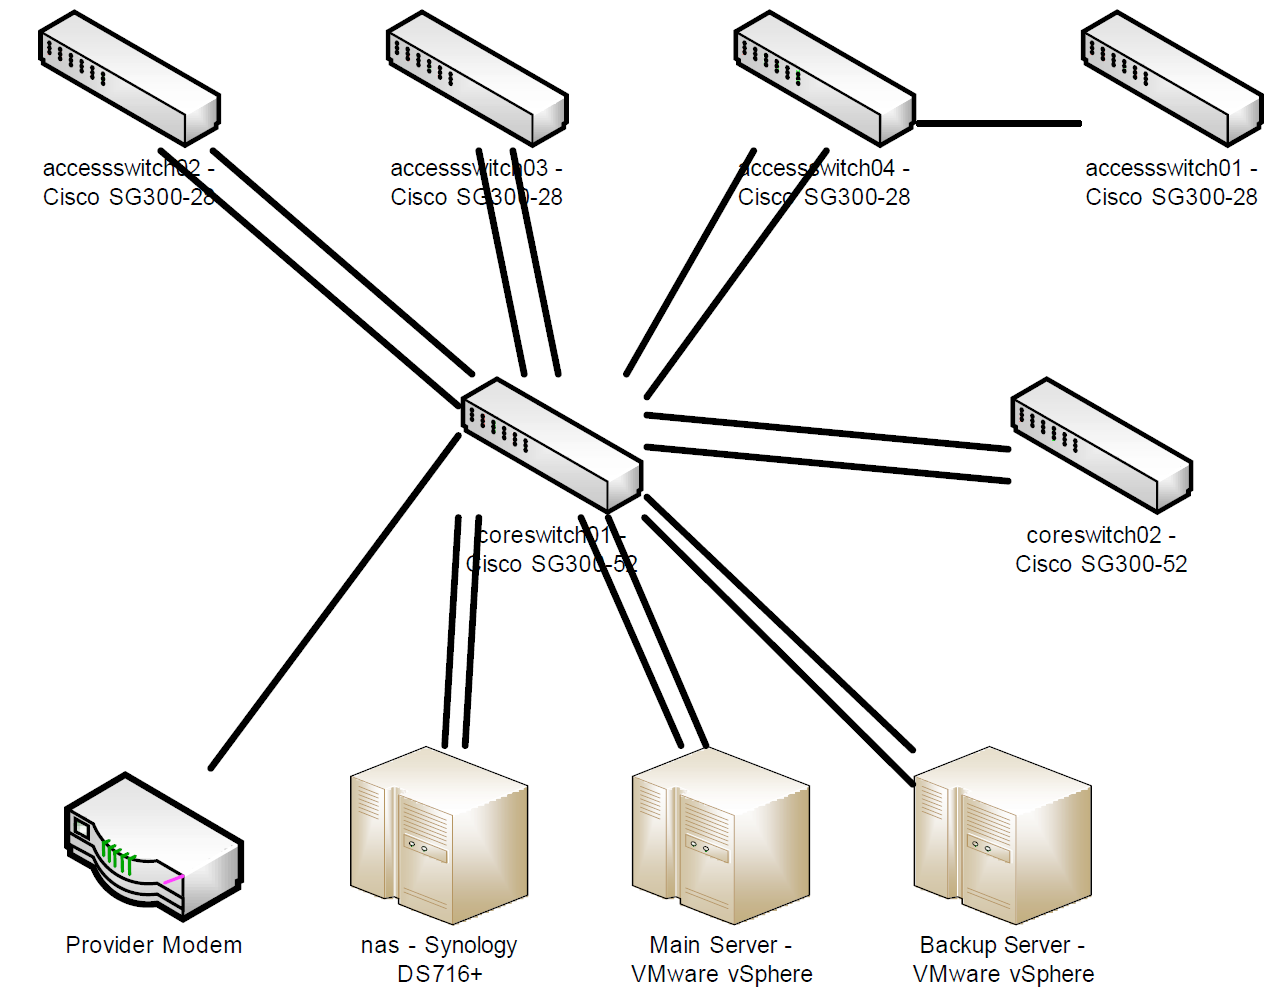
\includegraphics[width=0.8\textwidth]{BilderAllgemein/redundanz.png}
	\caption{Redundancy within the IT infrastructure}
	\label{img:redundanz_in_der_netzwerkinfrastruktur}
\end{figure}

To achieve redundancy between the switches, two instead of just one cable were laid. Each port on a switch, that was belonging to the same logical connection, was assigned to a \ac{LAG}. On the Cisco SG300 switches those \acp{LAG} are called port-channels. The configuration for those port-channels had to be the same on both switches. Furthermore the \ac{LACP} has been deactivated on both sides. The following listing shows the commands for the Cisco SG300 switch to achieve this configuration. Lines starting with an exclamation mark are comments.

\begin{lstlisting}
! assign the corresponding interfaces to a port-channel
coreswitch01(config)#interface gigabitethernet 49
coreswitch01(config-if)#channel-group 2 mode on
coreswitch01(config-if)#exit
coreswitch01(config)#interface gigabitethernet 50
coreswitch01(config-if)#channel-group 2 mode on
coreswitch01(config-if)#exit

! set the vlan configuration on the port-channel and not on 
! the interfaces
coreswitch01(config)#interface port-channel 2
coreswitch01(config-if)#description "to coreswitch02"
coreswitch01(config-if)#switchport mode trunk
coreswitch01(config-if)#switchport trunk allowed vlan add 10,
                        20,30
\end{lstlisting} 

Speaking of the redundant communication between core switch 1 and main server, as well as core switch 1 and backup server, all configuration had been made on the ESXi. On the core switch 1 itself no special configuration regarding \ac{LA} had to be made. \\
ESXi ensures redundancy, that means that all physical links except of one can fail. Moreover it makes load balancing between the physical links, so that the load is distributed equally upon all physical connections.

For the connection between core switch 1 and \ac{NAS} a \ac{LAG} has been created and \ac{LACP} enabled in passive mode. This is a requirement from the \ac{NAS} to get a working \ac{LA}. In addition, the port-channel connected to the NAS has been configured as an access port in VLAN 10. \\
The following listing shows the used commands to achieve that configuration on a Cisco SG300 switch.

\begin{lstlisting}
! assign the corresponding interfaces to a port-channel
coreswitch01(config)#interface gigabitethernet 5
coreswitch01(config-if)#channel-group 1 mode auto
coreswitch01(config-if)#exit
coreswitch01(config)#interface gigabitethernet 6
coreswitch01(config-if)#channel-group 1 mode auto
coreswitch01(config-if)#exit

! set the vlan configuration on the port-channel and not on 
! the interfaces
coreswitch01(config)#interface port-channel 1
coreswitch01(config-if)#description "to NAS"
coreswitch01(config-if)#switchport mode access
coreswitch01(config-if)#switchport access vlan 10
\end{lstlisting} 

\subsection{vSphere Network Configuration}

\begin{figure}[H]
	\centering
	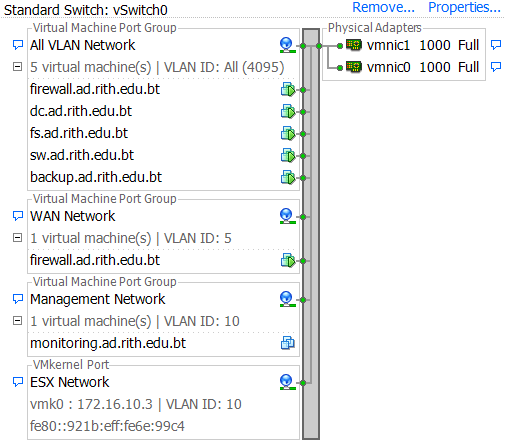
\includegraphics[width=0.8\textwidth]{BilderAllgemein/netzwerkkonfiguration_esxi.png}
	\caption{Network configuration ESXi main server}
	\label{img:netzwerkkonfiguration_esxi_main_server}
\end{figure}

Fig. \ref{img:netzwerkkonfiguration_esxi_main_server} shows the virtual network configuration of 1vSphere on the main server. As displayed, two physical network adapters are assigned to vSwitch0 in order to achieve redundancy and load balancing, as described in the previous chapter. Every network adapter works at 1 Gbps full duplex. \\
Due to the trunk, that has been configured on core switch 1, VLAN tagging has to be done on the vSphere too, in order to identify the different VLANs and successfully split the packets. For example core switch 1 is now tagging all packets that correspond to VLAN 10 with a 802.1Q tag containing the label 10. Only by doing this, the opposite side is then able to identify packets that belong to VLAN 10 by looking at the 802.1Q tag in the header of the IP packet. \\
For example the port group "Management Network", that can be seen in the picture, only handles packets with a 802.1Q tag that contain the VLAN ID 10.

In general two different connection types are distinguished. The VMKernel Port and the Virtual Machine Port Group. The former is a TCP/IP stack to manage traffic for the ESXi services vSphere Motion, iSCSI, NFS and host management. The latter is a virtual network interface that mainly offers three different options: define a specific VLAN ID, allow all VLAN IDs or allow no VLAN ID. \\
When a VLAN ID is specified on the virtual network interface only packets belonging to that VLAN are processed. Moreover the 802.1Q tag gets removed from the packet header. \\
When the virtual network interface is configured to allow all VLAN IDs, every packet containing a 802.1Q tag is processed. Therefore the operating system must take care of the separation of the packets concerning the VLANs. \\
If the virtual network interface is configured for no VLAN ID, only untagged packets will get processed by that interface.

The "ESX Network" of type VMkernel Port, as shown in the figure, is used to process the management traffic for the ESXi host. Only this VMkernel Port has an IP address assigned. The ESXi host is accessible via this configured IP address. \\
On the backup server this network was additionally used to access the iSCSI Target that is located on the NAS.

As seen in the figure the VMs "dc", "fs", "sw" and "backup" are assigned to the "All VLAN Network". That means that the VLAN separation has to be done within the operating system. In order to be able to use that, the network adapter for the VM has to be of the VMXNET3, as seen in figure \ref{img:network_adapter_vmxnet3}. 

\begin{figure}[h!]
	\centering
	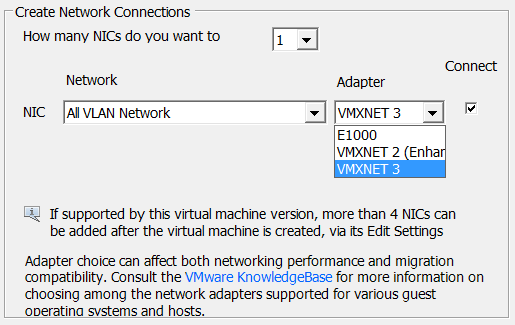
\includegraphics[width=0.6\textwidth]{BilderAllgemein/vmxnet3.png}
	\caption{Network adapter VMXNET3}
	\label{img:network_adapter_vmxnet3}
\end{figure}

After using VMXNET3 as network adapter type and allowing "All VLANs" on the network, the VLAN can be configured within the properties of the specific \ac{NIC} on the operating system. Fig. \ref{img:configuring_vlan_id_on_nic} shows the procedure in case of a Windows Server 2012 R2.

\begin{figure}[h!]
	\centering
	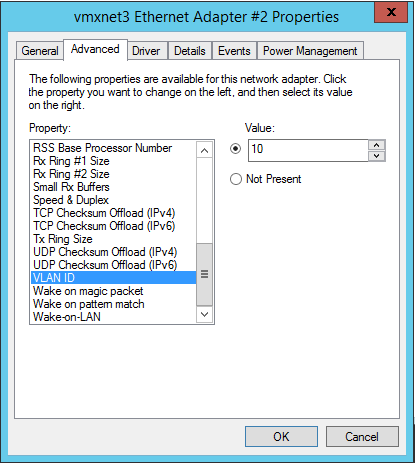
\includegraphics[width=0.6\textwidth]{BilderAllgemein/vmxnet3_properties.png}
	\caption{Configuring VLAN ID on NIC}
	\label{img:configuring_vlan_id_on_nic}
\end{figure}

The WAN interface of the VM "firewall" was connected to a network with the VLAN ID 5 and the LAN interface also the network with all VLANs allowed. 

The debian based VM "monitoring" was connected to a network for VLAN 10, because only one VLAN was needed and thus no VLAN configuration within the operating system had to be made.





\clearpage
%\chapter{Zusammenfassung und Ausblick}

\thispagestyle{standard}
\pagestyle{standard}

Zusammenfassend lässt sich sagen, dass die in dieser Arbeit erstellte IT Infrastruktur den aktuellen, zeitgemäßen Anforderungen entspricht. Auf Verfügbarkeit sowie Zuverlässigkeit wurde ebenso Wert gelegt wie auf die durchschnittliche Reparaturzeit. \\
Die Netzwerkinfrastruktur wurde soweit als möglich redundant geplant, des Weiteren ist eine durchdachte Backuplösung vorhanden. 

Im folgenden werden Erweiterungsvorschläge für die IT Infrastruktur angegeben, welche im Rahmen dieser Arbeit nicht durchgeführt werden konnten:

\begin{itemize}[noitemsep]
\item Erweiterung der Speicherkapazität des Backup Servers
\end{itemize}

%%%%%%%%%%%%%%%%%%%%%%%%%%%%%%%%%%%%%%%%%%%%%%%%%%%%%%%%%%%%%%%%%%%%%%%%%%%%%%%%%%%%%%%%%%%%%%%%%%%%%%%%%%%%
% LITERATURVERZEICHNIS

\interlinepenalty=10000 % Literatureinträge: Absätze zusammenhalten
\clearpage
\addcontentsline{toc}{chapter}{Literatur}
\singlespace
\bibliography{12bibliografie}
\interlinepenalty=100

%%%%%%%%%%%%%%%%%%%%%%%%%%%%%%%%%%%%%%%%%%%%%%%%%%%%%%%%%%%%%%%%%%%%%%%%%%%%%%%%%%%%%%%%%%%%%%%%%%%%%%%%%%%%
% ANHÄNGE

\begin{appendix}
%\include{Anhang_Mathematik}                 % A
%\include{Anhang_FormatDerParameterdateien}  % B
%\include{Anhang_Quelltexte}                 % C
%\include{Anhang_Datenblaetter}              % D
%\include{Anhang_Glossar}                    % E
\end{appendix}

\end{document}